\documentclass{article}

% NeurIPS 2026 submission style. The default option is the main-track,
% double-blind submission format (line numbers and anonymized author block).
\usepackage[preprint]{neurips_2026}

\usepackage[utf8]{inputenc}
\usepackage[T1]{fontenc}
\usepackage{hyperref}
\usepackage{url}
\usepackage{booktabs}
\usepackage{amsmath}
\usepackage{amssymb}
\usepackage{nicefrac}
\usepackage{microtype}
\usepackage{graphicx}
\usepackage{xcolor}

\title{Sparse Latent Dynamics for Financial Forecasting under Market Shifts}

\author{%
  Zhijie Jiang \\ \texttt{jian1223} \And
  Boyu Song \\ \texttt{songboy3} \And
  Shuo Liu \\ \texttt{liushu70} \And
  Yanming Zhao \\ \texttt{zhaoy439}
}


\begin{document}
\maketitle

\begin{abstract}
Financial returns are noisy and nonstationary, making it difficult for sequence models to generalize across market conditions. We propose to test whether sparse latent dynamics improve next-day ETF return forecasting relative to a standard gated recurrent unit (GRU). A GRU encodes a fixed historical window into a low-dimensional state; a learned state transition is regularized using a small polynomial library and a sparsity penalty. We will compare a direct GRU, a dense latent-transition model, and a sparse latent-transition model using chronological out-of-sample evaluation on four liquid ETFs. Performance will be assessed with forecast errors and regime-stratified diagnostics. We will also examine whether discovered terms remain stable when the encoder is held fixed. The primary contribution is a controlled evaluation of a dynamical inductive bias, not a claim to discover universal financial laws. Regime-conditioned transitions and more elaborate rolling retraining are optional extensions.
\end{abstract}

\section{Introduction}
Financial return predictability can change as volatility, monetary conditions, and cross-asset relationships evolve. Recurrent neural networks can learn nonlinear patterns from sequential observations, but may overfit historical relationships. Sparse identification of nonlinear dynamics (SINDy) offers a complementary structural assumption: a low-dimensional state transition may be approximated by a small number of candidate terms \citep{brunton2016}.

Our question is: \emph{Does a sparse latent-state transition improve out-of-sample financial forecasting relative to an otherwise comparable GRU, particularly during volatile market periods?} We do not assume that prices obey a deterministic ordinary differential equation. Instead, we test whether a parsimonious approximate transition is a useful predictive inductive bias.

\paragraph{Input and output.}
For trading day $t$, the input is a lookback window $X_t=[x_{t-L+1},\ldots,x_t]\in\mathbb{R}^{L\times d_x}$ of historical features observed by the end of day $t$, with $L=40$ initially. The output is a vector $\hat y_{t+1}\in\mathbb{R}^{N}$ predicting next-day close-to-close log returns for $N=4$ ETFs. The prediction time is after the close on day $t$; any feature not available by then is excluded.

\paragraph{Planned contributions.}
\begin{enumerate}
\item A reproducible chronological evaluation of GRU forecasting on a small multi-asset panel.
\item A controlled comparison of direct GRU, dense latent transition, and sparse latent transition, using the same sequence encoder where possible.
\item An analysis of forecast errors in calm versus stressed markets and of sparse-term stability in a fixed latent coordinate system.
\end{enumerate}

\section{Background and Related Work}
\paragraph{Financial sequence models.}
Fischer and Krauss \citep{fischer2018} evaluate LSTM models for financial prediction, motivating recurrent encoders for historical return sequences. Our study uses a GRU and emphasizes controlled comparisons rather than a more complex predictive architecture.

\paragraph{Sparse dynamics discovery.}
SINDy \citep{brunton2016} represents state changes using a sparse combination of candidate nonlinear terms. Champion et al.\ \citep{champion2019} jointly learn latent coordinates and governing equations with an autoencoder. SINDy-SHRED \citep{gao2026sindyshred} combines recurrent representations with sparse latent dynamics. Thus, combining recurrent learning and SINDy is \emph{not} claimed as a new general method; we examine its usefulness for nonstationary financial prediction.

\paragraph{Nonstationarity and alternative dynamics.}
Wang and Lera \citep{wang2026} study return prediction under shifting market regimes. Nguyen et al.\ \citep{nguyen2024} investigate neural ODEs for stock forecasting. Unlike a neural-ODE approach, our core method uses a one-day discrete transition and does not require a numerical ODE solver. We focus on whether sparsity provides benefits beyond adding a transition layer.

\section{Data}
\paragraph{Source and coverage.}
We downloaded daily adjusted closing prices and trading volumes for SPY, QQQ, TLT, and GLD from Yahoo Finance using \texttt{yfinance} with automatic price adjustment enabled. These ETFs provide exposure to U.S. large-cap equities, Nasdaq-100 equities, long-term U.S. Treasury bonds, and gold, respectively. Prices span January 4, 2010 to December 31, 2025. Computing daily log returns yields 4,023 observations from January 5, 2010 onward. The downloaded closing-price panel has no missing values across the four ETFs. Figure~\ref{fig:growth} summarizes their historical performance; normalized adjusted prices provide a common starting point for comparison.

\begin{figure}[t]
  \centering
  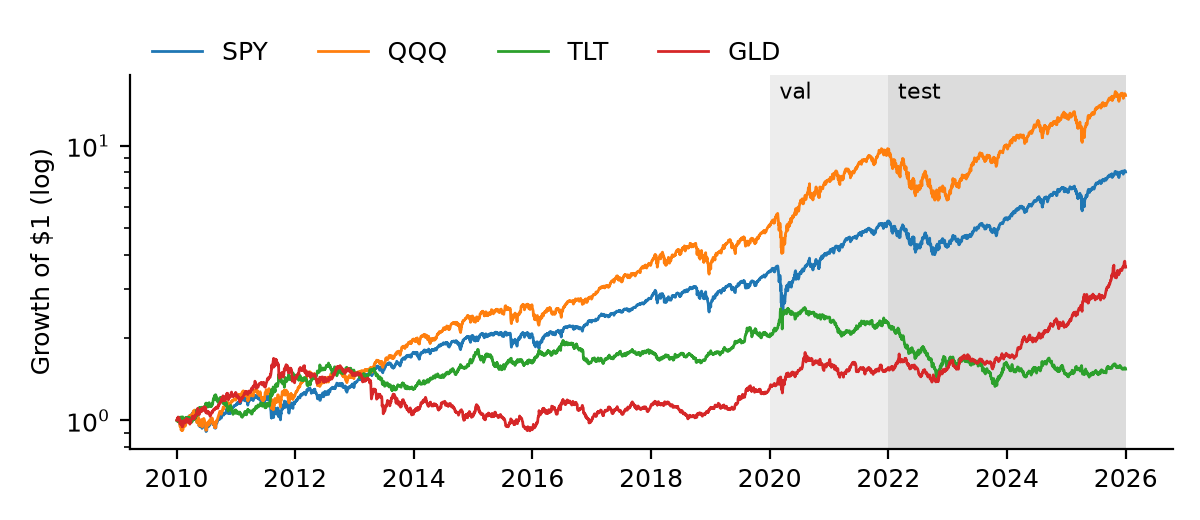
\includegraphics[width=0.9\linewidth]{figs/fig1_prices_splits.png}
  \caption{Historical value relative to an initial \$1, calculated by dividing each adjusted closing price by its initial value. The vertical axis is logarithmic. The unshaded region (2010--2019) is the training period; light-gray and darker-gray backgrounds identify the validation and test periods. The curves show cumulative performance, whereas our prediction targets are daily log returns.}
  \label{fig:growth}
\end{figure}

\paragraph{Inputs and prediction targets.}
For asset $i$, the target is $r_{t+1}^{(i)}=\log(P_{t+1}^{(i)}/P_t^{(i)})$, where $P_t^{(i)}$ is the adjusted closing price. Each input will contain 40 consecutive trading days of features available by the close of day $t$; the output will contain the four next-day log returns. Candidate features include historical returns, trailing volatility, momentum, and relative trading volume. Their exact definitions and lookback periods remain to be finalized using training and validation data.

\paragraph{Preprocessing and chronological splits.}
We will train on 2010--2019, select hyperparameters on 2020--2021, and evaluate final forecasts on 2022--2025. These periods contain 2,515, 505, and 1,003 daily return observations, respectively, before constructing model inputs. We will omit samples lacking sufficient feature history, rather than fill them using future observations. Scaling parameters and any optional clipping thresholds will be fitted on training data only. A proposed windowing rule assigns samples by target date and permits validation and test inputs to include earlier observations across split boundaries, since these would already be available at prediction time. Final usable sample counts will be recorded after feature construction. The exploratory figures include all periods; test prediction errors will be reserved for evaluation after model selection.

\paragraph{Volatility and evaluation regimes.}
To distinguish calmer from more volatile conditions, we compute SPY's trailing 20-day sample standard deviation of log returns, annualized by $\sqrt{252}$. The training-period 80th percentile defines a fixed threshold of approximately 17.4\%. Days above this threshold are labeled stressed; remaining days with available volatility estimates are labeled calm. The first 19 return observations are excluded from this classification. Figure~\ref{fig:volatility} shows substantial variation in volatility. This motivates reporting forecast errors separately across market conditions, rather than relying only on an aggregate error. These labels are evaluation groups, not separate training datasets. For next-day forecasts, we propose grouping errors by the regime observed at forecast time $t$.

\begin{figure}[t]
  \centering
  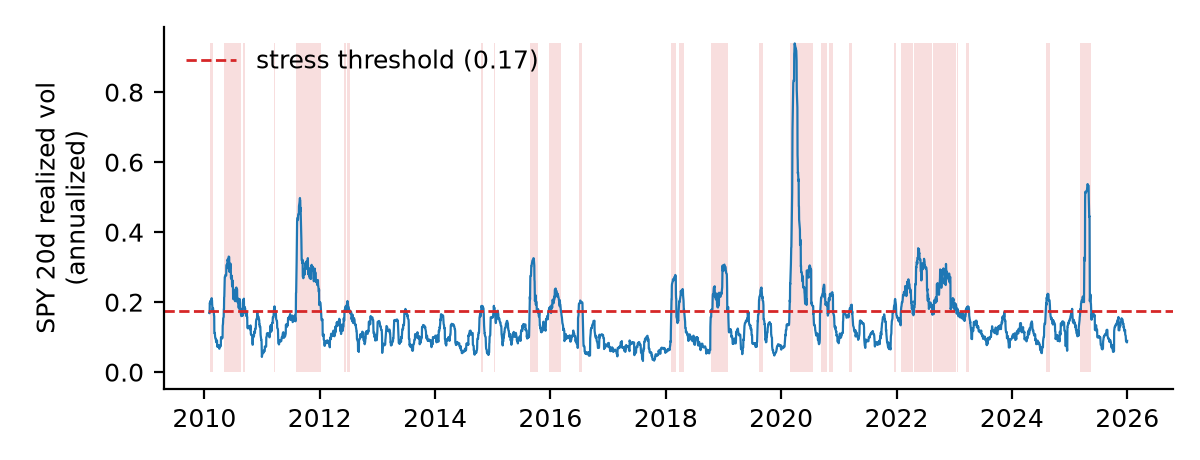
\includegraphics[width=0.85\linewidth]{figs/fig2_spy_vol_stress.png}
  \caption{SPY trailing volatility and the training-derived stress threshold. Shaded dates exceed the threshold. Volatility measures the variability of returns, not their direction; 17.4\% is an annualized volatility level, not a daily return.}
  \label{fig:volatility}
\end{figure}

\paragraph{Temporal dependence and modeling motivation.}
Figure~\ref{fig:acf} compares SPY return autocorrelations with those of absolute returns over lags of 1--30 trading days. At lag one, the values are approximately $-0.10$ and $0.31$, respectively. The more persistent positive autocorrelation in absolute returns is consistent with volatility clustering: large moves tend to occur near other large moves, even when their signs differ. This motivates investigating whether a sequence encoder can represent persistent market conditions. It does not establish that signed returns are predictably related to the past, or that the latent transition is sparse. Whether a sparse transition improves forecasts over direct-GRU and dense-transition baselines remains an empirical question.

\begin{figure}[t]
  \centering
  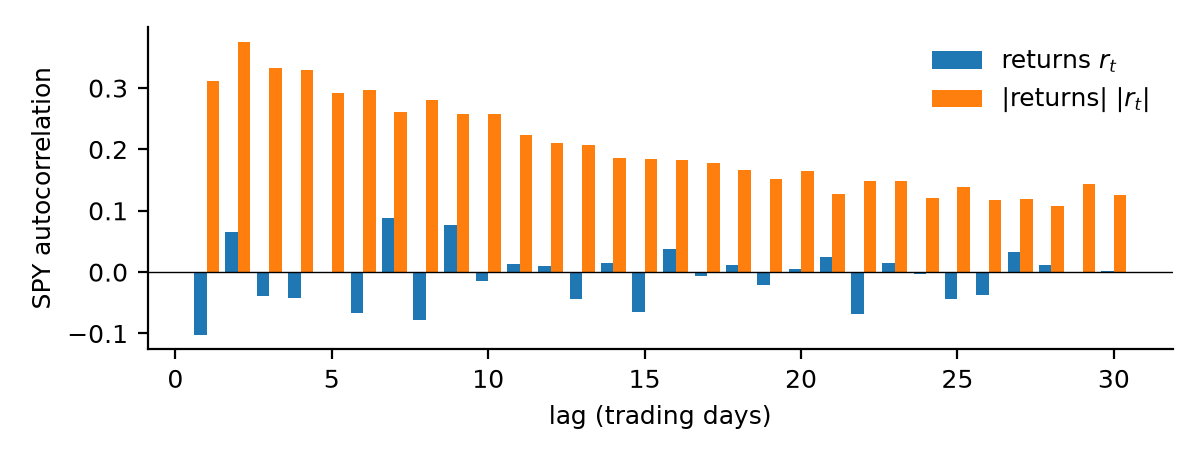
\includegraphics[width=0.85\linewidth]{figs/fig4_spy_acf.png}
  \caption{Autocorrelations of SPY daily log returns and absolute log returns. Each lag uses all available pairs separated by that many trading days. These are descriptive full-period estimates, without statistical significance intervals.}
  \label{fig:acf}
\end{figure}

\section{Model Architecture}
\paragraph{Shared GRU encoder.}
A one-layer GRU with 64 hidden units maps each input window to a latent state:
\begin{equation}
z_t=E_\theta(X_t)\in\mathbb{R}^{m},\qquad m=4.
\end{equation}
The same input features and encoder configuration will be used across learned baselines.

\paragraph{Three principal models for comparison.}
We will test 3 approaches on benchmarks: \emph{direct GRU} as blank control, \emph{dense-transition GRU} and \emph{SINDy}. The \emph{direct GRU} predicts $\hat y_{t+1}=h_\psi(z_t)$. The \emph{dense-transition GRU} uses
$\hat z_{t+1}=z_t+F_\phi(z_t)$ with a small MLP $F_\phi$, followed by $\hat y_{t+1}=h_\psi(\hat z_{t+1})$. The \emph{sparse-transition GRU} instead uses
\begin{equation}
\hat z_{t+1}=z_t+\Theta(z_t)\Xi,\qquad
\hat y_{t+1}=h_\psi(\hat z_{t+1}),
\end{equation}
where $\Theta(z_t)$ contains constant, linear, and quadratic monomial candidates and $\Xi$ is a trainable coefficient matrix. All models predict next-day returns; only the transition model differs.

\paragraph{Objective and identifiability.}
The sparse model minimizes
\begin{equation}
\mathcal L=\mathcal L_{\rm pred}
+\lambda_d\|E_\theta(X_{t+1})-\hat z_{t+1}\|_2^2
+\lambda_s\|\Xi\|_1
+\lambda_r\mathcal L_{\rm rec}.
\end{equation}
Here $\mathcal L_{\rm pred}$ is return MSE for comparing difference of predicted and actual returns, and $\mathcal L_{\rm rec}$ is an optional lightweight reconstruction loss to discourage meaningless latent space learning. The dense-transition baseline uses the corresponding transition-consistency term but no sparse coefficient penalty. Since jointly learned latent coordinates are not unique, we will not directly compare coefficients from independently retrained encoders. For interpretability tests, we will freeze a common encoder and fit or evaluate transitions in that fixed coordinate system.

\begin{figure}[t]
    \centering
    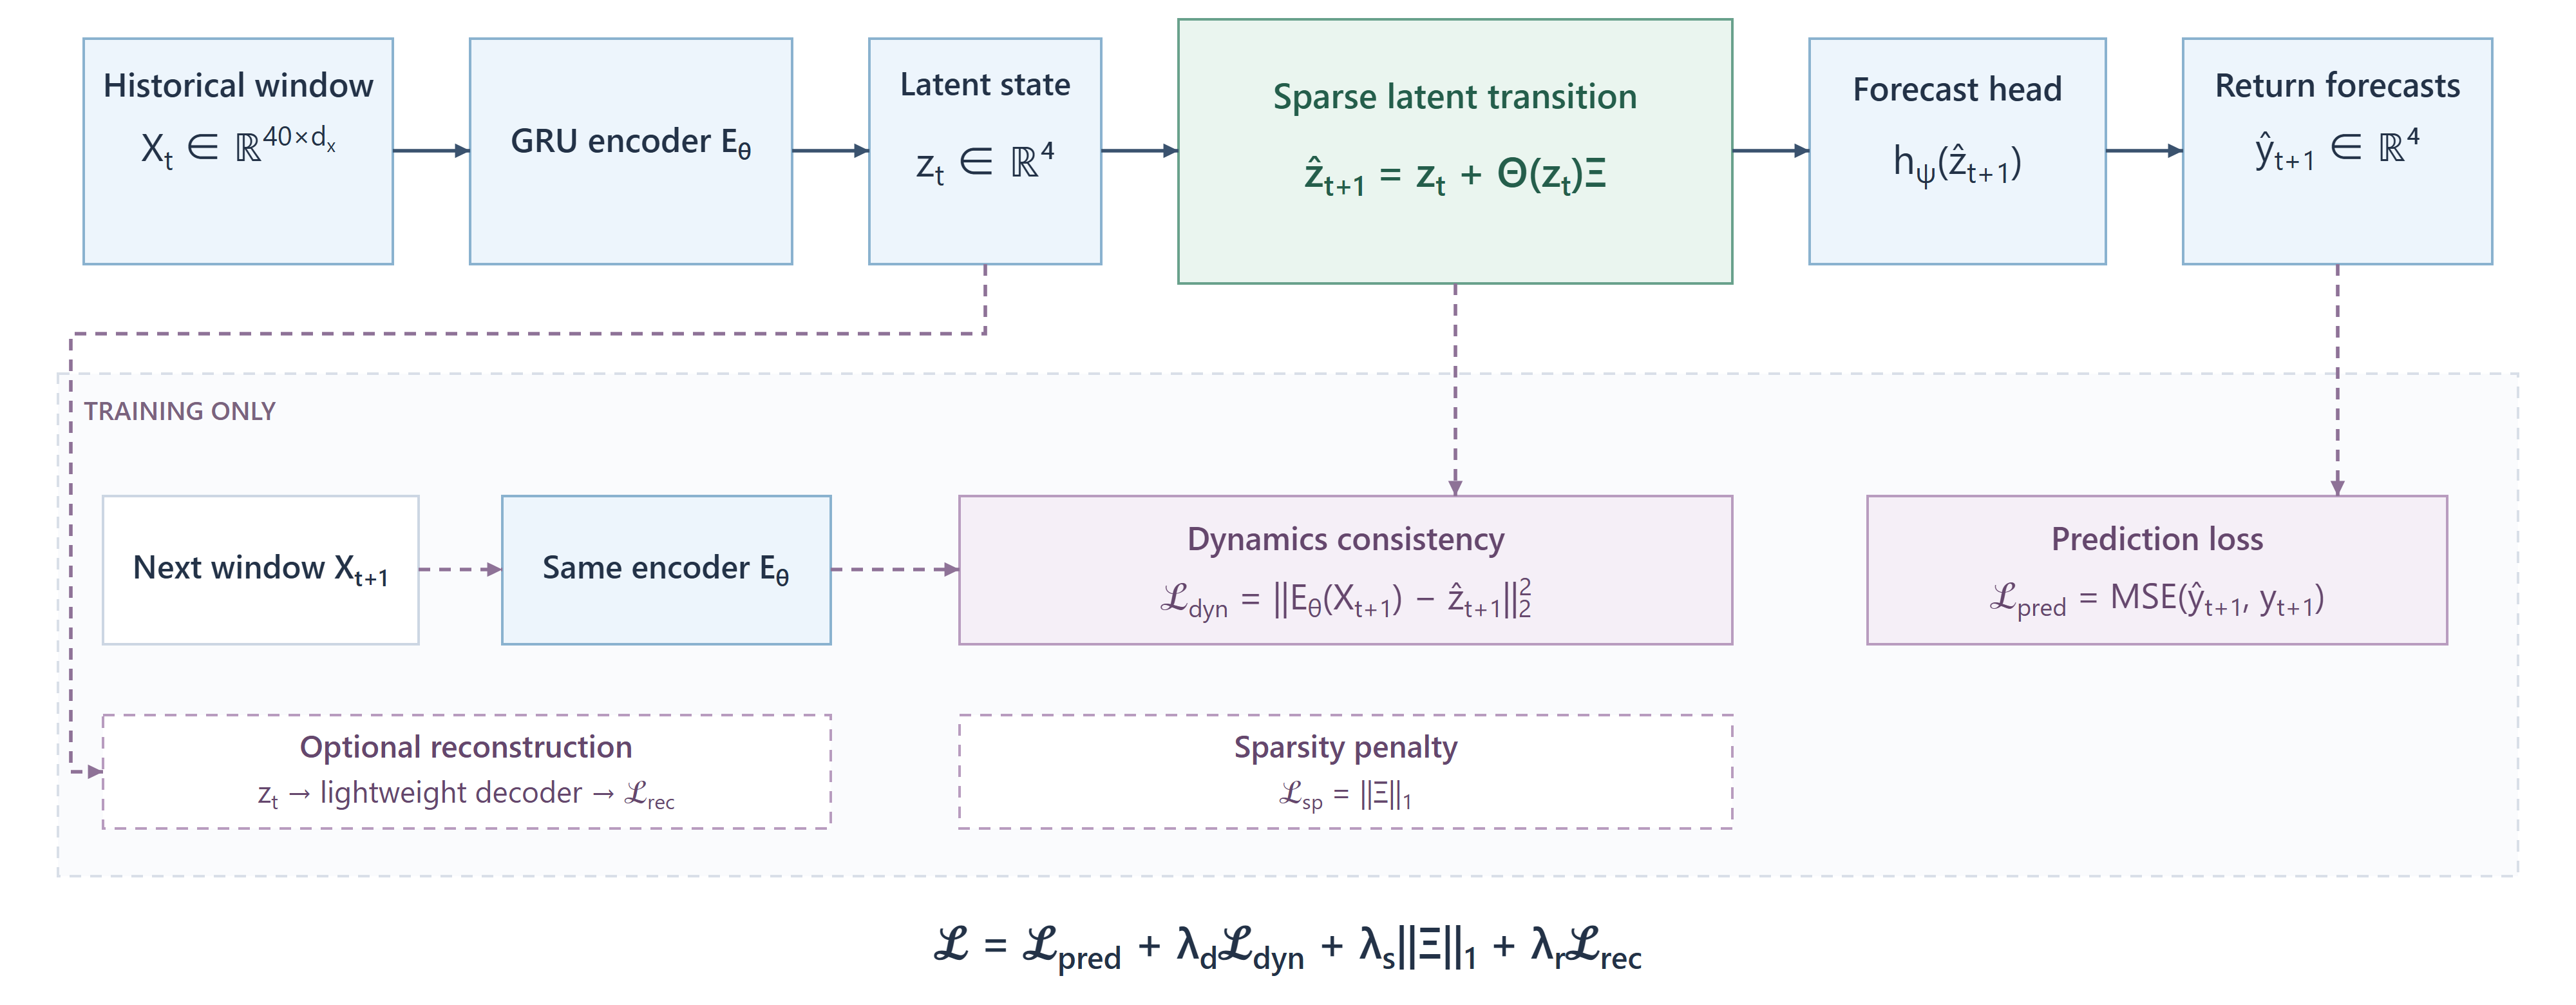
\includegraphics[width=\linewidth]{model_architecture_clean.png}
    \caption{Architecture of the sparse latent-transition GRU. A one-layer GRU with 64 hidden units and a linear projection encodes a 40-day historical feature window into a four-dimensional latent state. A residual sparse transition predicts the next latent state using 15 constant, linear, and quadratic candidate terms, with coefficient matrix $\Xi\in\mathbb{R}^{15\times4}$. The forecast head maps this predicted state to next-day log returns for SPY, QQQ, TLT, and GLD. Solid arrows denote the forward prediction path; dashed arrows denote training-only supervision. The next window is encoded using shared parameters to construct the dynamics-consistency target. Training combines return MSE, dynamics consistency, an $\ell_1$ coefficient penalty, and optional lightweight reconstruction. Future observations are used only as training targets; inference requires only $X_t$. The direct-GRU baseline predicts from $z_t$, while the dense-transition baseline replaces $\Theta(z_t)\Xi$ with a small MLP $F_\phi(z_t)$.}
    \label{fig:architecture}
\end{figure}

\paragraph{Implementation.}
We will use PyTorch, AdamW, early stopping on validation MSE, and a small validation-selected grid of $\lambda_d$ and $\lambda_s$. Initial settings are a 40-day window, 64 GRU hidden units, latent dimension four, and batch size 64; these may be adjusted using validation data. Neural ODEs and regime-specific coefficient mixtures are not required for the core project and would be attempted only with sufficient time.

\section{Proposed Evaluation}
\paragraph{Baselines.}
We will report a zero-return predictor as a simple financial benchmark and compare three learned models: direct GRU, GRU with a dense latent transition, and GRU with a sparse latent transition. A generic weight-decay control will be included if resources permit.

\paragraph{Primary metrics.}
The main metrics are next-day return MSE, MAE, and directional accuracy. We will also report errors separately for predeclared calmer and stressed periods. All models will use identical chronological splits and feature availability assumptions.

\paragraph{Dynamics diagnostics.}
We will report the number of retained polynomial terms, one-step latent transition error, and whether active terms are stable across time blocks when using a frozen encoder. Because sparsity alone does not establish economic interpretability, we will describe discovered terms as model-dependent relationships rather than governing laws.

\paragraph{Reproducibility and optional extensions.}
We plan to run three seeds for the main models and report means and variability. If the core experiments finish early, we may add one rolling-origin refit, a transaction-cost-aware illustrative backtest, or regime-conditioned transition coefficients. These are explicitly secondary and will not be necessary to answer the primary question.

\section{Ethical Considerations}
Historical market prediction can be mistaken for investment advice. We will present results as a methodological comparison, not a deployable trading strategy. Retrospective tests may overstate usefulness due to data selection, transaction costs, and changing market conditions. We will report negative results and uncertainty, and avoid interpreting latent equations as causal or universal financial laws. Public-data licensing and reproducibility will be documented.

\section{Work Division}
The project will be completed by four students. The following provisional assignments will be confirmed by the team:
\begin{itemize}
\item \textbf{Shuo Liu:} download and validate ETF data, implement chronological splits, prevent leakage, and prepare exploratory figures.
\item \textbf{Boyu Song:} implement the direct GRU and zero-return baseline, tune the GRU on validation data, and maintain reproducible training scripts.
\item \textbf{Zhijie Jiang:} implement dense and sparse latent transitions, consistency losses, and sparsity diagnostics.
\item \textbf{Yanming Zhao:} coordinate model comparisons, regime-stratified evaluation, plots, and assembly of the proposal and final report.
\end{itemize}
All members will review experimental design, test integrated code, interpret results, and contribute to writing. We plan a weekly team meeting and a shared repository with documented responsibilities.

\begin{thebibliography}{9}
\small

\bibitem[Brunton et al.(2016)]{brunton2016}
S.~L. Brunton, J.~L. Proctor, and J.~N. Kutz.
\newblock Discovering governing equations from data by sparse identification of nonlinear dynamical systems.
\newblock \emph{Proceedings of the National Academy of Sciences}, 113(15):3932--3937, 2016.
\newblock DOI: 10.1073/pnas.1517384113.

\bibitem[Champion et al.(2019)]{champion2019}
K.~Champion, B.~Lusch, J.~N. Kutz, and S.~L. Brunton.
\newblock Data-driven discovery of coordinates and governing equations.
\newblock \emph{Proceedings of the National Academy of Sciences}, 116(45):22445--22451, 2019.
\newblock DOI: 10.1073/pnas.1906995116.

\bibitem[Gao et al.(2026)]{gao2026sindyshred}
M.~L. Gao, J.~P. Williams, and J.~N. Kutz.
\newblock Sparse identification of nonlinear dynamics and Koopman operators with Shallow Recurrent Decoder Networks.
\newblock \emph{Proceedings of the National Academy of Sciences}, 123(16):e2508144123, 2026.
\newblock DOI: 10.1073/pnas.2508144123.

\bibitem[Fischer and Krauss(2018)]{fischer2018}
T.~Fischer and C.~Krauss.
\newblock Deep learning with long short-term memory networks for financial market predictions.
\newblock \emph{European Journal of Operational Research}, 270(2):654--669, 2018.
\newblock DOI: 10.1016/j.ejor.2017.11.054.

\bibitem[Wang and Lera(2026)]{wang2026}
Y.~Wang and S.~C. Lera.
\newblock Meta-learning for return prediction in shifting market regimes.
\newblock \emph{Journal of Financial Markets}, 79:101042, 2026.
\newblock DOI: 10.1016/j.finmar.2025.101042.

\bibitem[Nguyen et al.(2024)]{nguyen2024}
A.~Q. Nguyen, S.~Ha, and H.~Thai.
\newblock Phase space reconstructed neural ordinary differential equations model for stock price forecasting.
\newblock In \emph{Proceedings of the Pacific Asia Conference on Information Systems (PACIS)}, 2024.

\end{thebibliography}

\end{document}
